Qt is a framework that streamlines the development of high-performance, visually appealing and feature-rich GUI applications. It offers support for multiple languages such as C++, Python, and JavaScript, allowing developers to choose their preferred language. Thanks to the documentation and the large user base, there is a lot of support material to reference \cite{qt}.

With the \hyperref[sub:qt_designer]{Qt Designer}, developers can create GUI designs effortlessly. Designs can be created via drag-and-drop, which accelerates designing in Qt. It also enables developers to visualize what their application will look like in real-time \cite{qt}.

The feature-rich and vast knowledge base, coupled with its user-friendly design, made it an easy choice to use in this project to develop the applications.


\section{Qt Designer}
\label{sub:qt_designer}

This is a tool from the Qt framework that allows designing and building your GUI via drag-and-drop. It uses the what-you-see-is-what-you-get approach, where how it looks in the designer will be the same in the real application \cite{qt}.

Figure \ref{fig:qt_designer} shows the Qt Designer application, which consists of a main window to which widgets can be dragged from the left sidebar to place them in the application. If a layout is selected for the widgets, Qt will automatically fit them according to the layout, so ensuring that the widgets are properly aligned. In applications, it is important to know the hierarchy of the widgets. Qt Designer makes this process easy to figure out, the object window (on the top right) shows the hierarchy tree of the widgets. Making a widget a child of another widget can be achieved by dragging it into the parent widget. 

Not only can the content and placement of the widgets be adjusted, but it is also possible to set several properties of these widgets within Qt Designer (on the bottom right). This helps to see the changes immediately without having to start the GUI application. This is especially useful when changing the style or the layout of certain widgets, as these changes are immediately reflected in the designer.

Qt Designer makes Qt an attractive choice for developers looking to create a GUI application. The real-time visualization makes creating a GUI easy and efficient, making it possible to try out different looks of the application, resulting in a modern-looking design with minimal effort.

\begin{figure}
    \centering
    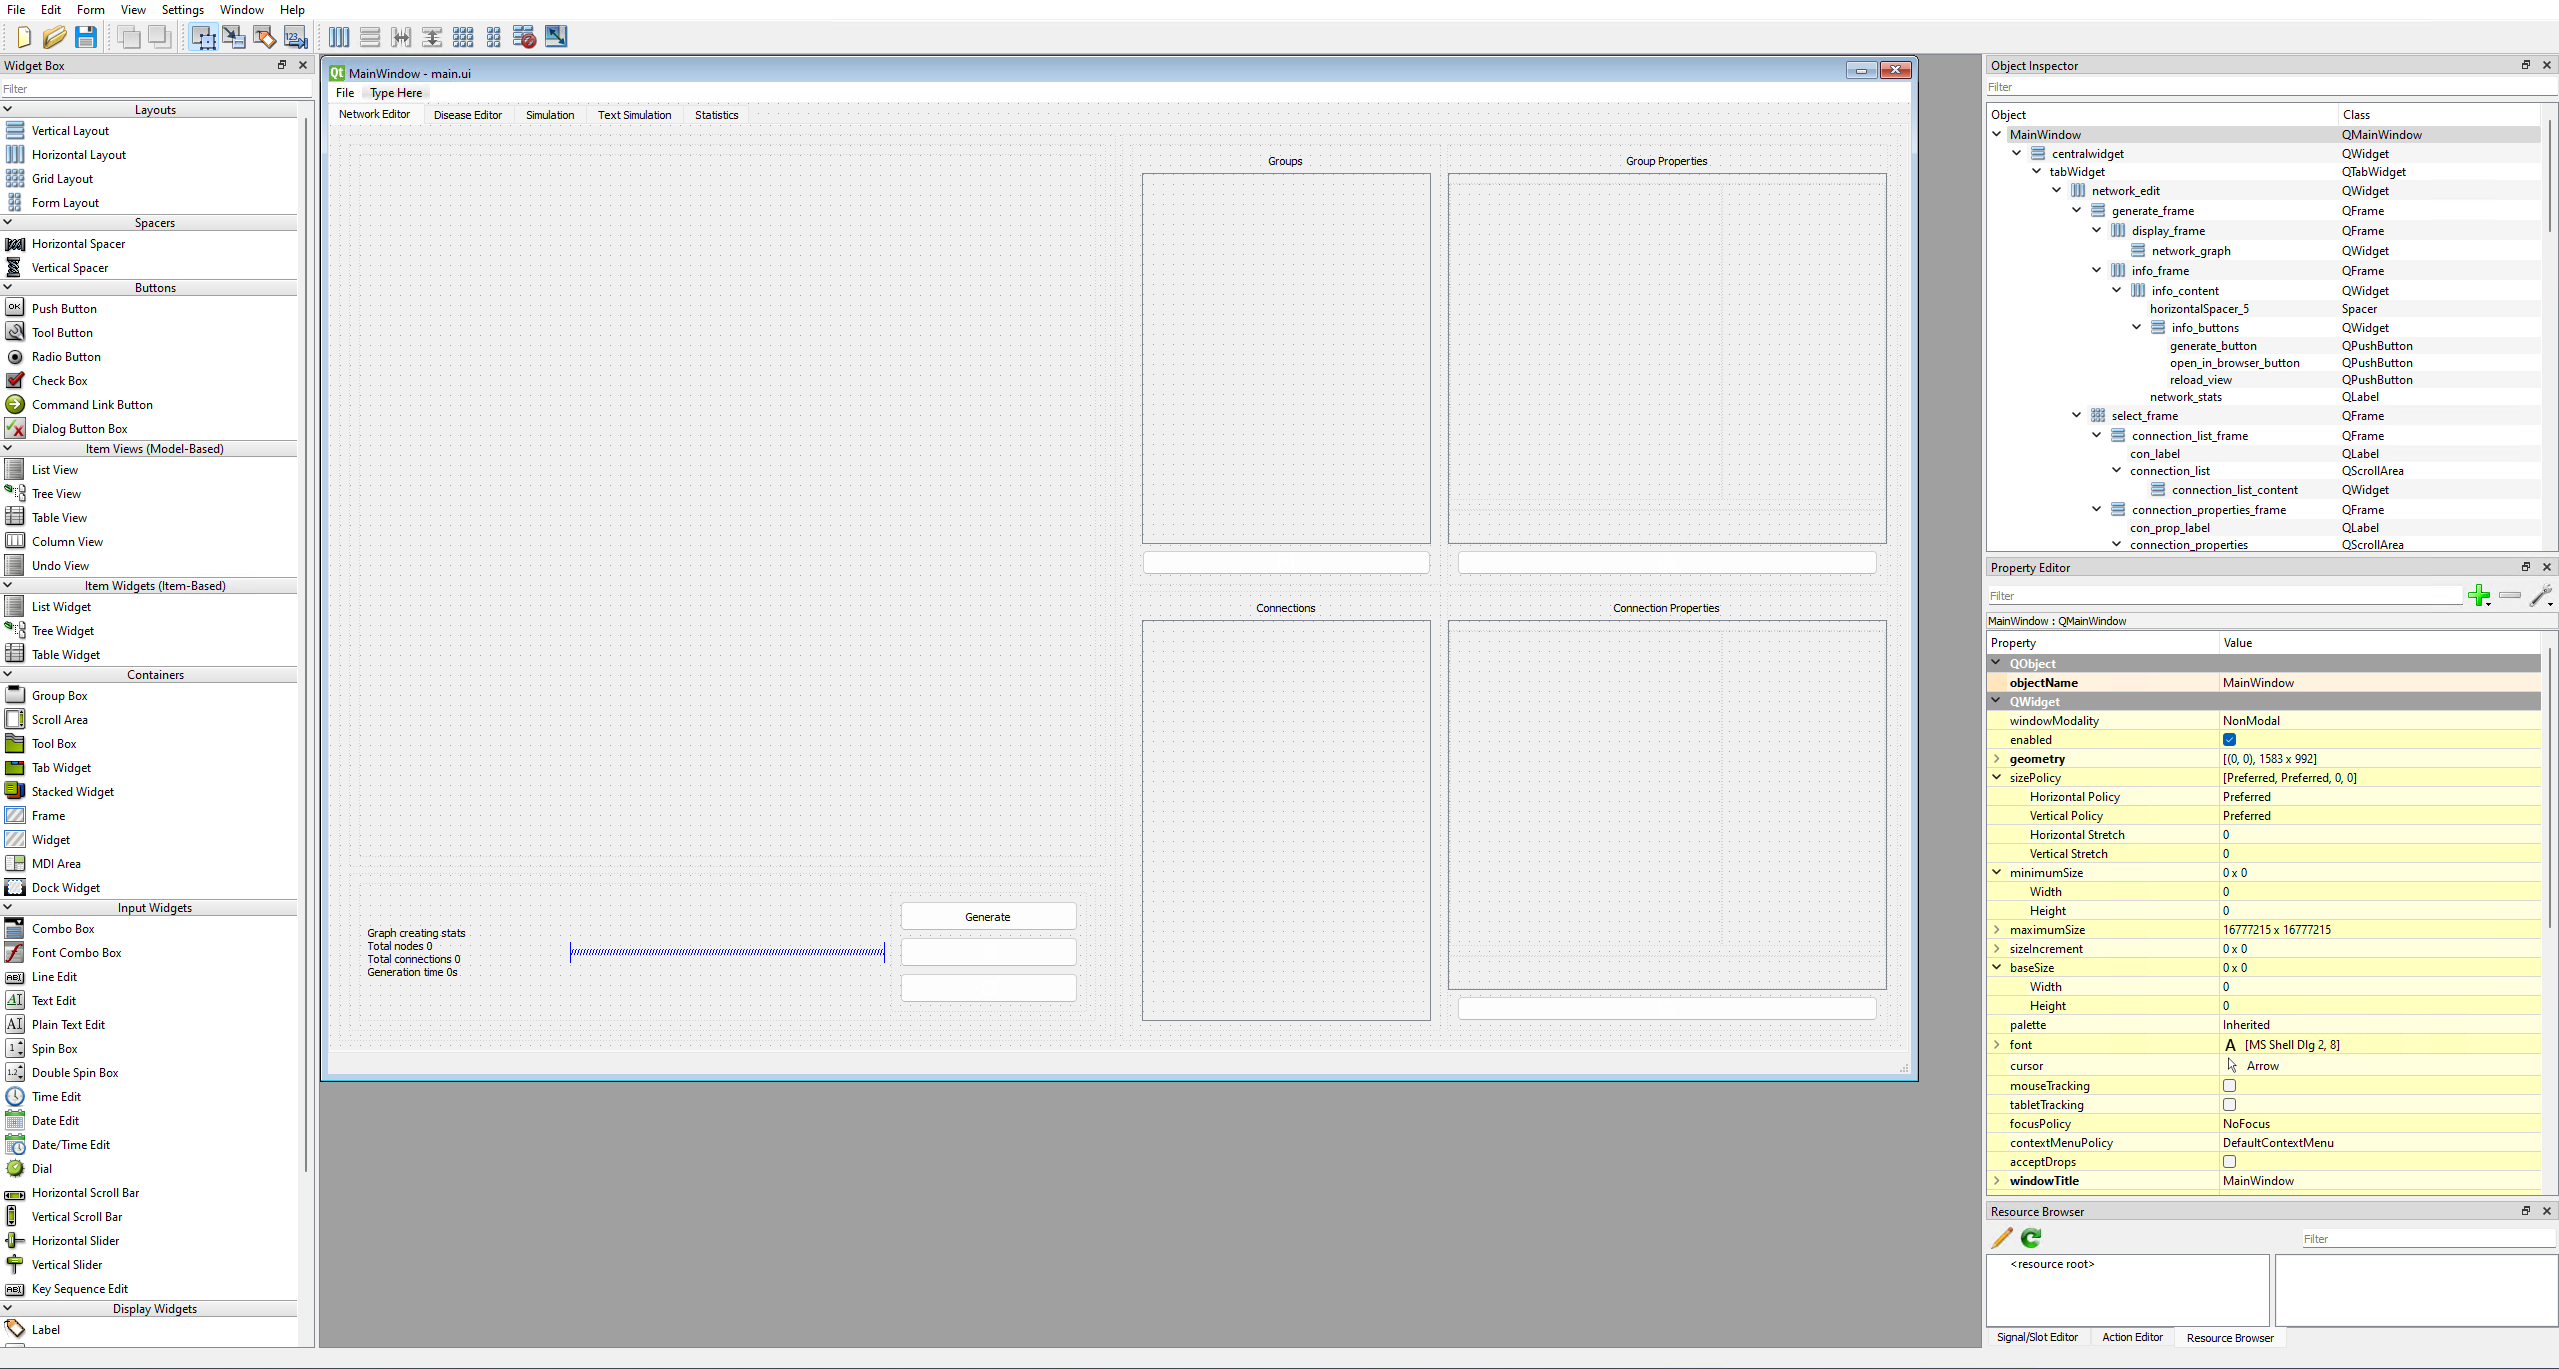
\includegraphics[width=0.8\linewidth]{images/qt_designer.png}
    \caption{Qt Designer}
    \label{fig:qt_designer}
\end{figure}

\section{PyQt}
\label{sub:pyqt}


Qt supports multiple programming languages to allow developers to choose their preferred language. This project was developed in Python, so PyQt was used. PyQt is a module that can be easily installed into the Python environment using pip. It contains all the add-ons that the C++ version of Qt also has. The add-ons can be used by importing the corresponding Python module. 

To develop an application in PyQt, the GUI can either be created using only the Python commands or with the help of the Qt Designer. The GUI created in the Qt Designer is saved in a \textt{.ui} file that can be loaded in the PyQt application \cite{pyqt}. Listing \ref{lst:pyqt_gui} shows how to load a \texttt{.ui} file into a simple application. 

Once a design is loaded into the application, it is easy to access the widgets that were created in the Qt Designer. To access and modify widgets created in the Qt Designer, they can be referenced using the ID associated with the widget in the designer. In Listing \ref{lst:pyqt_gui}, the widget created in the Qt Designer has the ID \textit{myLabel}. Depending on the type of widget, different functions are available, in this case the widget is a label, which contains the \textit{setText} function to change the text it displays. Other widgets, such as a frame widget, offer different functions. 

After a design is loaded, it is possible to add more widgets to it. For example, if buttons need to be created dynamically. This allows developers to create the default design of their application in the Qt Designer and dynamically change the content or arrangement of the widgets in the application. The ease of access to the objects created by the Qt Designer helps to improve the readability and simplicity of the application code.

\begin{lstlisting}[language=python, caption={Simple Qt GUI application}, label={lst:pyqt_gui}]
from PyQt5 import QtWidgets, uic
import sys
class GuiApplication(QtWidgets.QMainWindow):
    def __init__(self):
        super(GuiApplication, self).__init__()
        uic.loadUi('basic.ui', self)
        self.myLabel.setText('Changed text')
        self.show()

app = QtWidgets.QApplication(sys.argv)
window = GuiApplication()
app.exec_()
\end{lstlisting}

\section{Signals and Slots}
\label{sub:signals}

In GUI programming, it is often necessary to execute functions when, for example, a button is pressed. Other frameworks use callbacks to achieve this functionality; Qt uses the signals and slots mechanism. The signal is emitted by an object when its internal state changes. The slot is the function that will be executed once the corresponding signal is emitted. A signal can have multiple slots connected to it, which are executed one after the other. The signal-slot mechanism is independent of the GUI event loop and is executed immediately after a signal is emitted \cite{qt}.

Each signal has a \textit{.connect(Slot slot)} function that is used to connect the signal to a slot. For example, a button in Qt has three signals: \textit{clicked}, \textit{pressed}, and \textit{released}. In order to connect a function to the button, the following command has to be used: \textit{example\_button.clicked.connect(slot\_function)}. Now, when the button is clicked by the user in the GUI, the \textit{slot\_function} is executed \cite{pyqt}.

%TODO ein bsp aus dem code mit signal/slot

\subsection{Thread communication}
\label{sub:thread_communication}

In general, it is bad practice to have a thread modify GUI widgets to ensure separation of concerns. If this thread were killed prematurely, it could result in an unexpected GUI state that could lead to errors. Or, if the main thread changed the structure of the GUI widgets before the thread could add the desired widgets, this would also lead to errors. To solve this issue, the signals and slots mechanism is ideal for this situation. Instead of letting a thread handle the widget creation, the thread just sends the widget data back to the main thread, which then adds or modifies the widgets. This way, the integrity of the GUI can be maintained because the main thread retains control over widget manipulation, ensuring consistent and expected behavior \cite{qt}.

In listing \ref{lst:pyqt_thread_comm}, a simple thread is displayed. It has two signals: the finished signal and the result signal. The result signal has a string as a parameter that is sent along with the signal to the slot that will be executed. The thread creates a string that should be displayed using labels, to change the text property of the label the string is emitted using the result signal. This way, the widget modification is done only in the main thread \cite{pyqt}.

\begin{lstlisting}[language=python, caption={Thread example}, label={lst:pyqt_thread_comm}]
import sys
import time
from PyQt5.QtCore import pyqtSignal, QThread
class Worker(QThread):
    finished = pyqtSignal()
    result = pyqtSignal(str)

    def __init__(self):
        super().__init__()

    def run(self):
        time.sleep(2)
        result_data = "My Custom Data"
        self.result.emit(result_data)
        self.finished.emit()
\end{lstlisting}


\section{Abblication views}
\label{sub:thread_views}
The GUI application of the created app, contains five tabs/views, each with a different use:
\begin{description}
    \item[Network Editor] In this view, the user can create a network consisting of nodes and connections and view it in a 3D space.
    \item[Disease Editor] Allows to create the disease that are used for the simulation in the created network.
    \item[Simulation] The Simulation view embeds the webpage used for simulation. It displays the network and its state during the simulation, allowing the user to observe the behavior of the disease in the network.
    \item[Text Simulation] If the network is too big or a large number of simulation cycles are required, which makes using the visual simulation impractical, this text-based simulation can be used instead. It provides the same functionality for controlling the simulation and saving statistics as the visual simulation.
    \item[Statistics] This view embeds the webpage used to display the saved statistics. It can be used to view graphs for the various stats saved during simulations to help analyze the results.
\end{description}

%TODO mention custom QSS?